\section{Motivation}

The effects of climate change increase in severity every year. From 1980 to present, the global temperature anomaly - defined as the difference between the current average global temperature and the average temperature from 1951-1980 - has steadily increased to 1.02 $^{\circ}$C.  With a growing interest in reducing the global carbon footprint, comes a bevy of new research into sustainable energy, and the next generation of nuclear reactors.

One such class of reactors are the high temperature gas-cooled reactors, or HTGRs.  While HTGRs can have a variety of fuel forms, this work is concerned with pebble-bed reactors.  Pebble-type fuels generally consists of a sphere of graphite, approximately the size of a billiard ball, embedded with tri-structural isotropic (TRISO) particles.  In addition, the pebbles are able to be refueled while the reactor is online, reducing the need for planned shutdowns.

The next generation of nuclear reactors also include designs smaller than the conventional Light Water Reactor (LWR) seen in the USA today.  So-called Small Modular Reactors, or SMRs, are small enough to be shipped, reactor pressure vessel and all, in a standard shipping truck or train.  Owing to their small size, they are also easier and cheaper to manufacture.  SMRs can be deployed in a variety of new settings, such as isolated towns or work sites, or stationed together in one plant to fill the role of a single larger reactor.

This work used a pebble-bed HTG-SMR as a starting point, and modeled a generic 200MWth reactor based on existing designs - the Sangamon200. Then it scaled down to a target size - a 20MWth pebble bed HTGR.  Reactors with a capacity of 70 MWth or less are called microreactors, and can be deployed in areas where only a small amount of power is needed, used for research and testing, or be used to supply heat for other industrial processes, such as producing hydrogen.

Down-sized modular reactors, such as SMRs or microreactors, have a few inherent safety benefits over their larger cousins, which also prompts their development.  The smaller scale of the reactor pressure vessel (RPV) makes the large active cooling loops of contemporary commercial nuclear reactors unneccesary.  For smaller reactors, decay heat can be removed with passive systems that rely on natural convection and surface heat transfer after something such as a station black-out (SBO).  When power is supplied, supplementary fans and surface coolers can aid heat removal \cite{reutler_advantages_1984}.

The 20MWth model, which will hereafter be referred to as Sangamon20, is of a highly simplified design, which can be used in future testing and analysis.



\section{Objectives}

This work briefly describes a 200 MWth pebble-bed HTGR SMR, inspired by concepts from the PBMR and X-energy reactors, henceforth named Sangamon200.  After establishing the larger model as a baseline, a scaled-down 20 MWth model, Sangamon20, is designed, and is the focus of this work.

A series of tests modify the original Sangamon20 design, and analyses their effect on $k_{eff}$, fast and thermal flux, and neutron energy spectrum.  These modifications include heterogenizing versus homogenizing the pebble centers, applying a 6-point symmetry to the core (using one-sixth to approximate the entire core), and re-assigning pebble fuel compositions to test randomness and pebble mixing.  Additionally, the isotopic compositions for all pebble burnups are supplied, and trends over increasing burnup are discussed.

\section{Background}
\subsection{The High Temperature Gas Cooled Reactor: Beginnings and Concepts}

High temperature gas cooled reactors, or HTGRs, are a prominent Generation IV reactor design which often uses helium as a coolant, and graphite as a moderator in thermal designs.  Their fuel form uses TRISO particles, which consists of a small kernel of fuel, less than half a millimeter across, surrounded by layers of carbon and silicon carbide to protect the fuel kernel and prevent the leakage of radioisotopes.  These TRISO particles are then embedded in graphite to form a usable fuel element.  In prismatic HTGRs, the graphite is in the shape of hexagonal columns.  In pebble-bed reactors, the graphite is in the shape of spheres - around the size of a billiard ball.  Many of these pebbles are loaded into the core, and slowly move through the bottom in a manner similar to grain in silos.

HTGRs, however, are not a new concept.  Preliminary concepts for a gas-cooled reactor were created as early as 1942.  Farrington Daniels - more commonly known for his work in chemistry and solar power technology - is attributed with establishing the first theoretical designs.  A professor from the University of Wisconsin, Professor Daniel's work with Oak Ridge National Laboratory (ORNL) nailed-down the most basic characteristics of the HTGR.  The choice of helium for coolant, graphite for moderator, the direct gas turbine cycle, and the use of uranium or thorium carbides for fuel all came from his work \cite{simnad_early_1991}.

\begin{figure}[h!]
\centering
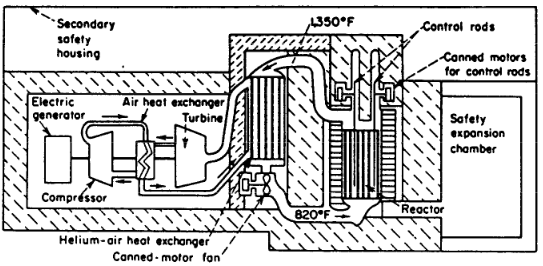
\includegraphics[width=0.6\linewidth]{figures/daniels-1}
\caption{Side-View of the 1955 Daniels' Concept, \cite{simnad_early_1991}}
\label{fig:daniels-1}
\end{figure}
\begin{figure}[h!]
\centering
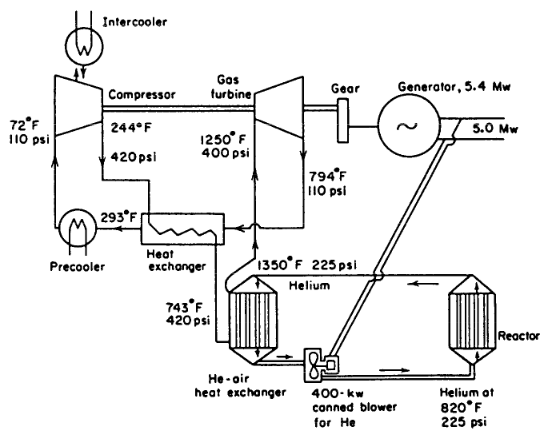
\includegraphics[width=0.6\linewidth]{figures/daniels-2}
\caption{Diagram of Coolant Flow in the 1955 Daniel's Concept, \cite{simnad_early_1991}}
\label{fig:daniels-2}
\end{figure}

Figures \ref{fig:daniels-1} and \ref{fig:daniels-2} show the 1955 design proposed by Professor Daniels.  Like many modern modular reactor plant designs, Professor Daniels suggested that the reactor be mostly underground.  A key difference between the Farrington Daniels designs and modern HTGRs is the fuel form.  While modern designs use TRISO particles embedded in graphite, the Daniels' design uses solid graphite blocks, with channels for both coolant and fuel.  Within the fuel channels, fuel was loaded in either a pellet or cartridge form, both a mixture of 10$\%$ uranium dicarbide and graphite powder.  In addition to these fuel channels, the design included an outer ring of graphite reflector in which thorium was used to breed $^{233}U$.  Control rods were made of boron-containing molybdenum.  Additional safety rods made of the same material were held above the core by steel wires that would melt in the case of an accident, dropping the safety rods into the core \cite{simnad_early_1991}.

\subsection{Earliest Operational HTGRs}

The earliest operational HTGRs: the AVR, from Germany; Dragon, operating in the UK; and Peach Bottom 1, which operated in the US came online in the 1960s \cite{beck_high_nodate}.

\subsubsection{Dragon}

The Dragon prismatic HTGR was a test reactor operated in Winfrith, UK, from 1964 to 1975, making it the oldest of the reactors discussed in this chapter.  It operated at inlet and outlet temperatures of 350 \textdegree C and 750 \textdegree C and 20MWt \cite{beck_high_nodate}.  Dragon's main purpose was to test reactor materials, with an emphasis on fuels.  It originally used uranium and thorium as fuel, but switched to a purely uranium-based fuel with a lower enrichment later in life.  The fuel elements themselves were similar in shape to the Daniels' design - hexagonal prisms with fuel rod channels.

Contrary to the fuel philosophy seen today, Dragon originally allowed fission products to be released from fuel elements into the circulating helium coolant.  The fission products would then be purged from the helium.  However, Dragon later switched to a coated-particle fuel when it became clear that having such large fission product releases would be difficult to manage \cite{simnad_early_1991}.

\subsubsection{Peach Bottom 1}

Peach Bottom 1 was operated from 1966 to 1974, by the Philadelphia Electric Company.  It was the first operational HTGR in the US, and the first to produce electric power.  It was slightly larger than Dragon, at a nameplate capacity of 115 MWt/40MWe and a slightly lower operating temperature range at 327\textdegree  C to 700\textdegree  C inlet to outlet \cite{beck_high_nodate}.  Like Dragon, Peach Bottom 1 was a prismatic reactor; however, Peach Bottom used coated uranium and thorium carbide particles from the beginning.  The original fuel used a single coating of pyrolytic carbon.  However, after multiple fuel failures, Peach Bottom upgraded to bistructural isotropic, or BISO, fuels by adding an additional layer.  Peach Bottom would later upgrade the fuel once again by adding a silicon carbide layer, forming TRISO particles \cite{beck_high_nodate}.  One operational benefit of upgrading to TRISO particles from BISO particles was that the superior fission product retention meant that Peach Bottom 1 could remove the helium purging systems.  In addition to the inner fuel region, Peach Bottom, like the Daniels' design, bred $^{233}U$ in an outer region using thorium.

Beyond changing the number and materials for fuel coatings, the experiences in Peach Bottom 1 helped to develop HTGR fuel elements.  Operators saw that they could dilute the fuel with graphite moderating material more so than other diluents.  This has the advantage of saving fuel material, improving heat transfer, and reducing radiation damage.  Additionally, operational experience showed that, in order to prevent the creation and buildup of $^{236}U$ and $^{237}Np$, which are neutron poisons, the $^{235}U$ and $^{233}U$ should be kept separate \cite{simnad_early_1991}.

In the end, Peach Bottom 1 closed when it was determined to be uneconomical.

\subsubsection{AVR}

The Arbeitsgemeinschaft Versuchsreaktor (AVR) was an experimental pebble-bed reactor operated in the Jülich Research Center from 1967 to 1988.  It had a capacity of 46 MWt/15MWe, with inlet and outlet temperatures of 275\textdegree  C and 950\textdegree  C \cite{beck_high_nodate}.  In fact, the AVR reached the highest operating temperatures of any commercial nuclear plant.  Like the others in this early time period, the AVR used a combination of uranium and thorium fuels, though it began with bi-structural isotropic (BISO) particles.  The core held around 100,000 graphite pebbles, almost a third of which had fuel in them.

Despite not being built for experimental purposes, the AVR still housed many experiments that improved our body of knowledge on HTGR technology.  During the first few years of its life, the goal of the AVR was to demonstrate that it was a reliable technology.  After this inital period, the AVR shifted focus to allow various experiments.

In the initial phase they needed to show that the reactor could operate safely, could control the core power and temperatures, safely shutdown, and remain sub-critical for long periods of time.  This proved to be quite the undertaking, as the AVR shifted from highly enriched to low enriched fuel over time, which caused a large variety in fuel pebble compositions, on top of the range of compositions inherent to a multi-pass pebble cycle.

The AVR also provided data to validate models of pebble-bed reactors, and conducted an experiment to better characterize the radial distribution of temperatures in the core.  A number of marked pebbles were loaded into the core, each housing a series of wires that would melt at a certain temperature, the lowest being 655\textdegree  C, the highest 1280\textdegree  C.  The pebble positions were tracked with pebble flow data, and when the spheres were ejected they were examined to determine what temperatures the pebbles had experienced.  Despite the outlet temperature being determined to be 950\textdegree  C, multiple pebbles experienced a temperature greater than or equal to the 1280\textdegree C maximum temperature in the melt wires.  It was noted that these pebbles went through a zone with a spike in local power density, which could account for the temperature spike \cite{noauthor_results_1990}.

The AVR also demonstrated the inherent safety of HTGR reactors in accident scenarios by purposefully causing failures of the active cooling system.  In the first, the coolant blowers were shutoff, and no shutdown rods were inserted while operating at full power.  The operators additionally shut the main circuit valves to prevent natural circulation to regions outside the active core.  Overall, the changes to core temperatures were unremarkable.  The hottest regions cooled, while the coldest regions warmed up.  Additionally, due to negative temperature feedback coefficients, the reactor power immediately declined in response to the "accident".  The temperature slowly rose to 2 MW again over 24 hours, only to level out around 300 kW.  A further test provided data on loss of coolant and depressurization accidents.  As before, the core temperature changes were not drastic.  The upper core region was seen cooling, while the lower, originally cooler core region slowly rose in temperature.  This experiment's data was used to validate HTGR computer models, which allowed the results to aid in the analysis of other HTGRs \cite{noauthor_results_1990}.

Beyond accident safety, the AVR allowed for testing and demonstration of the safety qualities of TRISO and BISO fuel elements; especially relating to high temperature tolerance, and fission product retention.  Initial tests were conducted with BISO based pebbles, then later transitioned to TRISO, then to low-enriched-uranium (LEU) TRISO pebbles.  The TRISO-LEU pebbles were shown to have good fission product retention compared to their BISO-based predecessors, based on the the activity of samples taken from the circulating helium.  Beyond radioisotopes being directly released into the coolant gas, the AVR also showed that in order to accurately characterize the source term of am HTGR pebble bed reactor, one must take the dust from the pebbles into account.  Dust from the pebbles bumping and scraping against each other was found deposited on reactor surfaces in the primary loop.  It was found that 60 kg of dust had accumulated by the end of the reactor's life, which averages to 3 kg of dust each year.  Measurements of specific activity in the dust showed that the activities of $^{137}Cs$, $^{134}Cs$, $^{131}I$, $^{90}Sr$, and $^{60}Co$ were on the order of $10^6 Bq g^{-1}$.  Even though there is relatively little dust, the activity of this dust is fairly high, especially compared to the activity of the coolant gas \cite{noauthor_results_1990}.

***(I'm going to include here the two tables comparing the activities of the coolant gas and dust activities.  However, the one for gas is (reasonably) by volume, while the dust is by mass.  Should I use the density of helium at operating temperature to convert the gas activity to be in Bq/g, and make a new table (citing my source), or leave as-is?)***

\begin{figure}[h!]
\centering
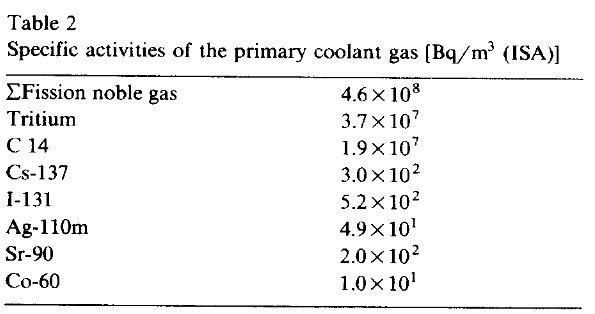
\includegraphics[width=0.7\linewidth]{figures/gas-act-tab}
\caption{Helium Coolant Specific Activities \cite{noauthor_results_1990}}
\label{fig:gas-act-tab}
\end{figure}
\begin{figure}[h!]
\centering
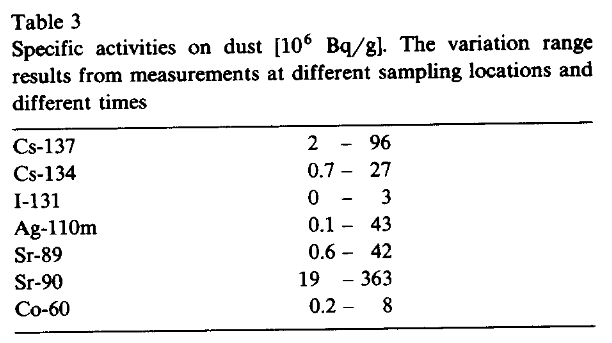
\includegraphics[width=0.7\linewidth]{figures/dust-act-tab}
\caption{Pebble Dust Specific Activities \cite{noauthor_results_1990}}
\label{fig:dust-act-tab}
\end{figure}


\subsection{Serpent}
Serpent 2 is "a multi-purpose three-dimensional continuous-energy Monte Carlo particle transport code" \cite{noauthor_serpent_nodate} from the VTT Technical Research Center of Finland.  The first iteration, Serpent 1, began development in 2004.  The development of Serpent 2 is presently on-going.  Serpent 2 has three main applications: traditional reactor physics, coupled multi-physics, and neutron and photon transport.  